\section{Applications}
\label{s:numerics}

\begin{figure}%[H]
\centering
%  \begin{tabular}{c c c c c c}
 (a) 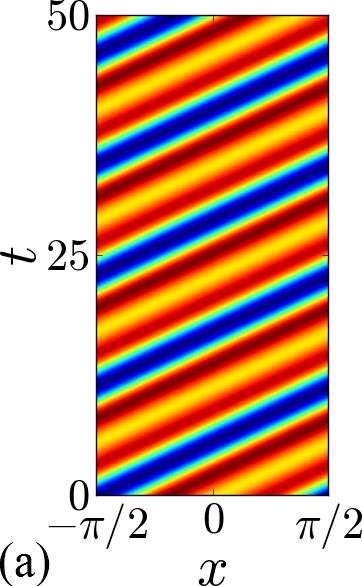
\includegraphics[width=0.12\textwidth]{2modes-conf-reqv} %&
 (b) 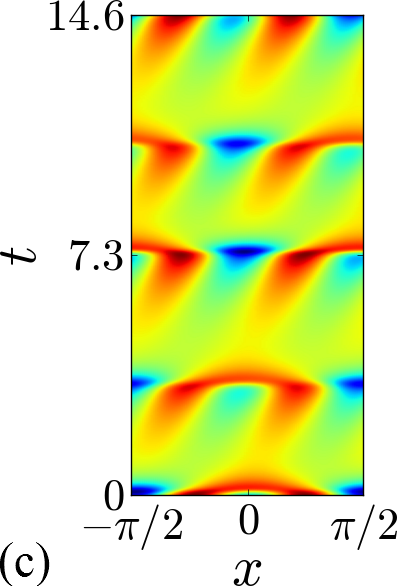
\includegraphics[width=0.12\textwidth]{2modes-conf-rpo} %&
 (c) 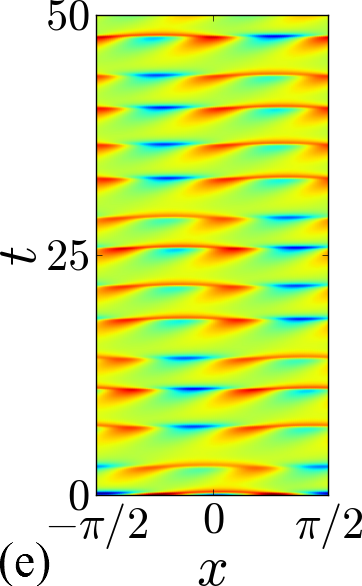
\includegraphics[width=0.12\textwidth]{2modes-conf-ergodic} \\ %&
 (d) 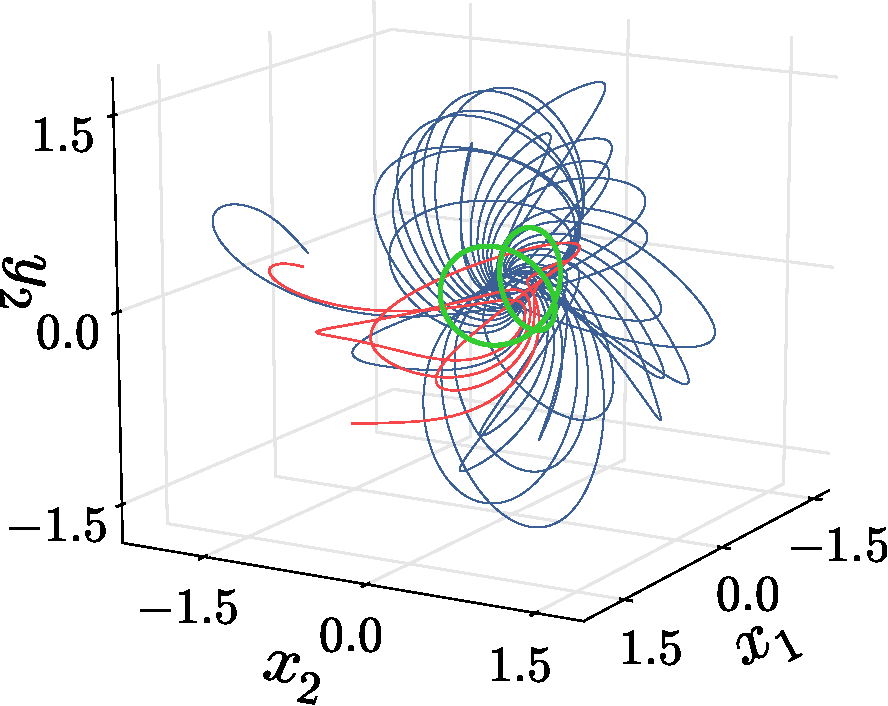
\includegraphics[width=0.45\textwidth]{2modes-ssp} \\ %&
 (e) 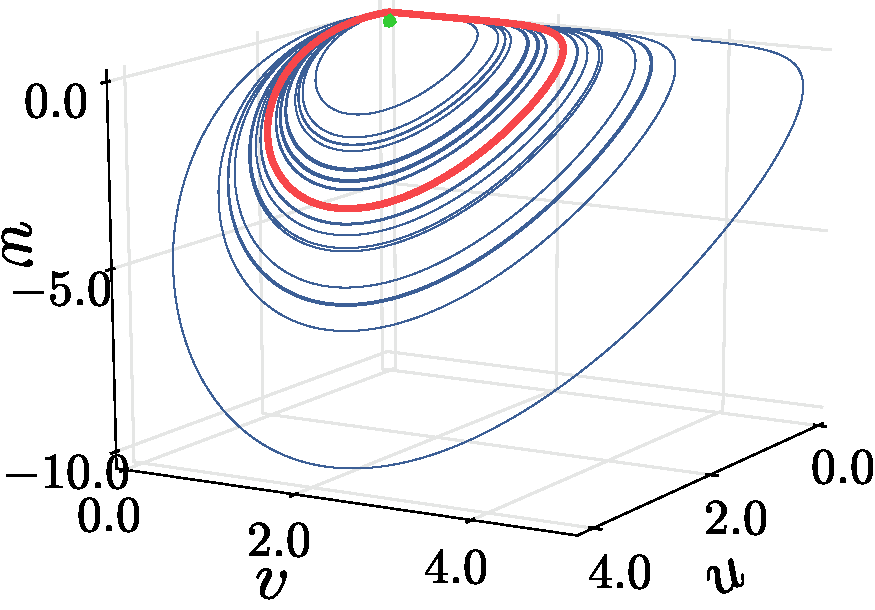
\includegraphics[width=0.21\textwidth]{2modes-invpol} %& 
 (f) 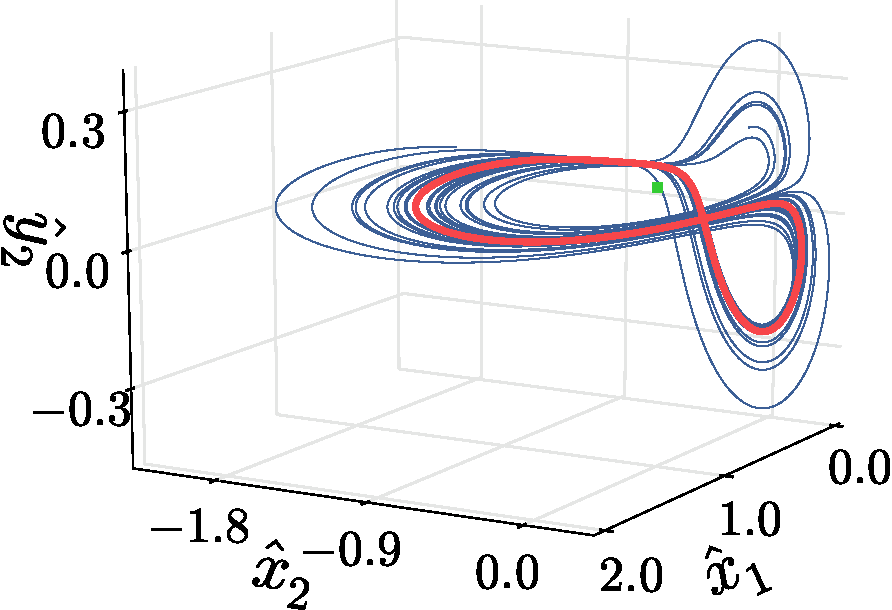
\includegraphics[width=0.21\textwidth]{2modes-sspRed} %\\
%  \quad (a) & \quad (b) & \quad (c) & (d) & (e) & (f)
%  \end{tabular}
% (d) 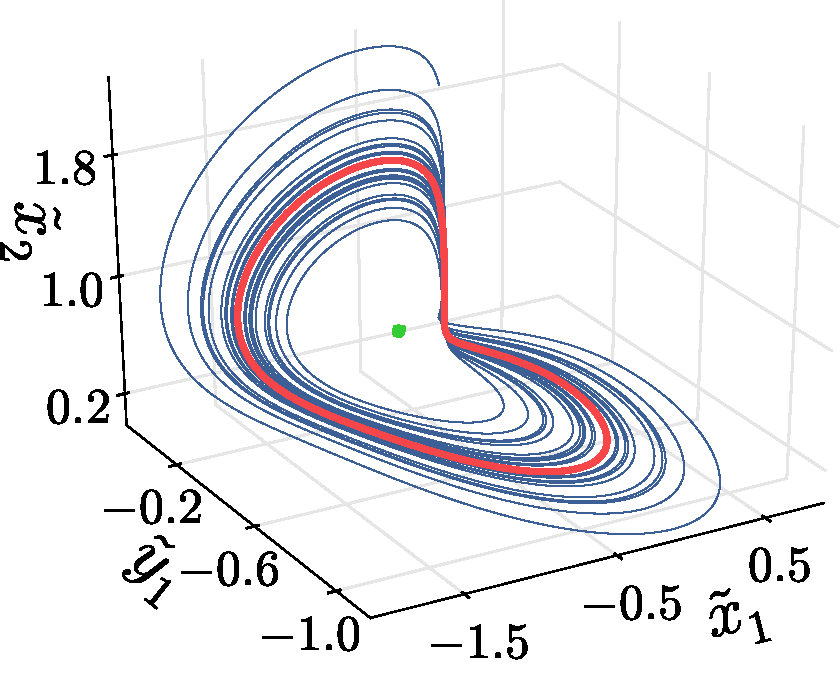
\includegraphics[width=0.20\textwidth]{2modes-sspRed2}
% (d) 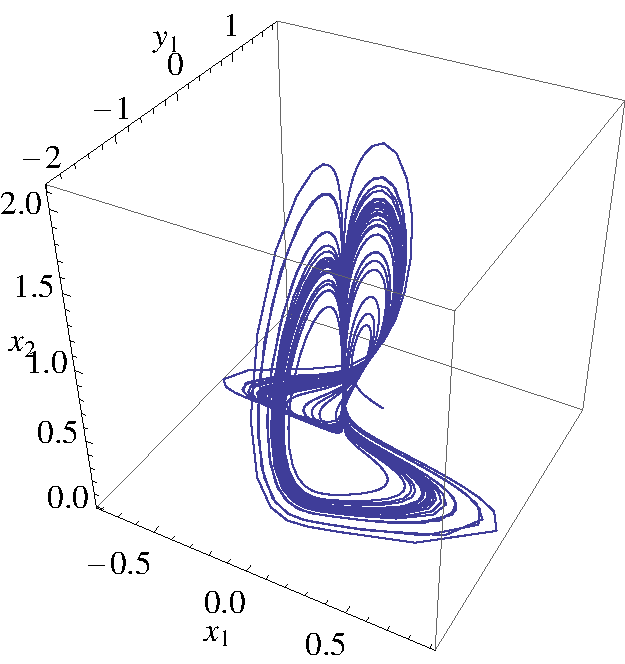
\includegraphics[width=0.20\textwidth]{2modesSliceIntFM2}
\caption{(Color online) 
The \reqv\ (a), two repeats of \rpo\ \cycle{01} (b), and a typical
ergodic trajectory of the \twomode\ system in the configuration
space; same trajectories colored green, red and blue respectively 
in a 3D projection of four-dimensional \statesp\ (d), invariant 
polynomials (e), and the first Fourier mode \slicePlane\ (f).}
\label{fig:Set1}
\end{figure}
\ES{2014-05-15}{I have replaced the second-mode slice, double-angled figure in \reffig{fig:Set1}(b)
with one resulting by integrating on the $(0,0,1,0)$ slice, for consistency with
panel (c). I hope Burak will replace it with a publication quality figure of the same
representation. The trick of angle doubling will be introduced in its own section.
}
\begin{table}
	\caption{Parameters used here to study the \twomode\ system.}
	\begin{tabular}{c|c|c|c|c|c|c|c|c|c}
	% after \\: \hline or \cline{col1-col2} \cline{col3-col4} ...
	 $\mu_1$ & $\mu_2$ & $e_1$ & $e_2$ & $a_1$ & $a_2$ & $b_1$ & $b_2$ & $c_1$ & $c_2$ \\
	\hline   
	 -2.8	& 1		  & 0	  & 1	  & -1	  & -2.66 & 0	  & 0 	  & -7.75 & 1	  \\
	\end{tabular}
	\label{tab:pars}
\end{table}
To illustrate the \mslices\ on the \twomode\ system we choose a simple 
set of parameters for which we observe interesting dynamics. These
parameters are listed in \reftab{tab:pars}. With this set of parameters,
we can write \twomode\ ODEs \refeq{eq:DangSO2} in terms of three parameters $\{ \mu_1, c_2, a_2 \}$:
\bea
\label{eq:DangSO2set1}
  \sspC_1 &=& \mu_1 \,z_1 - z_1|z_1|^2 +c_1\,\overline{z}_1\,z_2
  \continue
  \sspC_1 &=& (1-\ii)\,{z_2}+a_2\,z_2|z_1|^2+\,z_1^2
\,,
\eea
Note that by setting $b_2 = 0$, we send the \reqv\ at $\invpol = (0,-\mu_2/b_2,0,0)$ to infinity. Moreover, \refeq{PKinvEqs5a} yields $\tilde{v} = (\mu_1 + \tilde{a}_1 \tilde{u})/(\mu_2 + \tilde{a}_2 \tilde{u} - \tilde{u} \tilde{b}_1)$. Substitution into \refeq{PKinvEqs5b} allows one to solve for a single variable. By solving \refeq{PKinvEqs5} with the parameter set \reftab{tab:pars},
we get two real roots, with non-negative $u$ and $v$: %the \eqva\ of the system in the invariant polynomial basis \refeq{Dang86(1.2)PK} as
\[
	\invpol_{\EQV{}} = (0,0,0,0)^T %\qquad \mbox{(double)}
\]
which is a double root and corresponds to an equilibrium of \refeq{eq:DangSO2}, and
\[
			 \invpol_{\REQV{}{}} = (0.193569,0.154131,-0.149539,-0.027178)^T\,,
\]
which is a relative equilibrium. In real representation, a
representative point on  \REQV{}{} may be chosen as
\[
  \left(x_1, y_1, x_2, y_2\right) = \left(0.439966, 0, -0.386267, 0.070204\right)
\]
We visualize the dynamics of the \twomode\ system in four different representations: 3D projections of the four-dimensional real valued \statesp and invariant polynomials, in the 3D \slicePlane\ and on the 2D configuration space plots on which the color-coded field $u(\conf, \zeit)$ is defined as follows:
\bea
	u(\conf, \tau) &=& \sum_{k=-2}^{2} \sspC_k(\zeit) e^{i k \conf}\, ,
	\continue && \mbox{where} \, \sspC_{-k} = \sspC_k^* \, \mbox{and} \,
	\sspC_0 = 0 \, .
\eea
\refFig{fig:Set1} shows the only \reqv , \rpo\ \cycle{01} and an ergodic trajectory of the \twomode\ system in the four different representations we described above. Note that translation of the \reqv\ in the configuration space \reffig{fig:Set1} (a), corresponds to the \SOn{2} rotations in the \statesp\ of Fourier modes in \reffig{fig:Set1} (d) (green curve) and these orbits correspond to a single point in the symmetry reduced representations of \reffig{fig:Set1} (e, f). Note also that the \rpo\ \cycle{01} translates/rotates as it advances in configuration space (\reffig{fig:Set1} (b)) and in the equivariant \statesp\ \reffig{fig:Set1} (\reffig{fig:Set1} (d)), whereas in the symmetry reduced plots (\reffig{fig:Set1} (e, f)), it closes onto itself after one period.

\subsection{Finding Cycles}

The simple structure of the symmetry reduced dynamics allows us to determine the 
\rpo s of the \twomode\ system by means of a Poincar\'e section and a return map. We illustrated this procedure in \reffig{fig:psectandretmap}. Starting with an initial
point close to the \REQV{}{}, we computed a long ergodic trajectory of the symmetry reduced \twomode\ system by integrating \refeq{e-so2red1stmode} (blue curve in \reffig{fig:psectandretmap} (a)) and recorded its intersections (marked with red in \reffig{fig:psectandretmap} (a)) with the Poincar\'e section (transparent plane in \reffig{fig:psectandretmap} (a)), which includes the \REQV{}{} and the imaginary part of its unstable stability eigenvector (one of the green arrows in \reffig{fig:psectandretmap} (a)). We then projected these intersections onto a
basis $(v_1, v_2)$, which spans the Poincar\'e section, and fit cubic splines to this set of points, see \reffig{fig:psectandretmap} (b). The return map of arclengths from the origin which is set to \REQV{}{} in \reffig{fig:psectandretmap} (b), is unimodal with an sharp cusp located at its critical point, shown in \reffig{fig:psectandretmap} (c). Note that the region corresponds to the neighborhood of the \reqv\ $s = (0, 0.6)$ is never visited once the flow leaves it and falls onto the chaotic attractor. For this reason, we re-drew this return map after discarding the data corresponding to the initial transients in \reffig{fig:psectandretmap} (d). We use this return map to determine the accessible \rpo s  with their respective binary symbol sequences.

\begin{figure}
\centering
  (a) 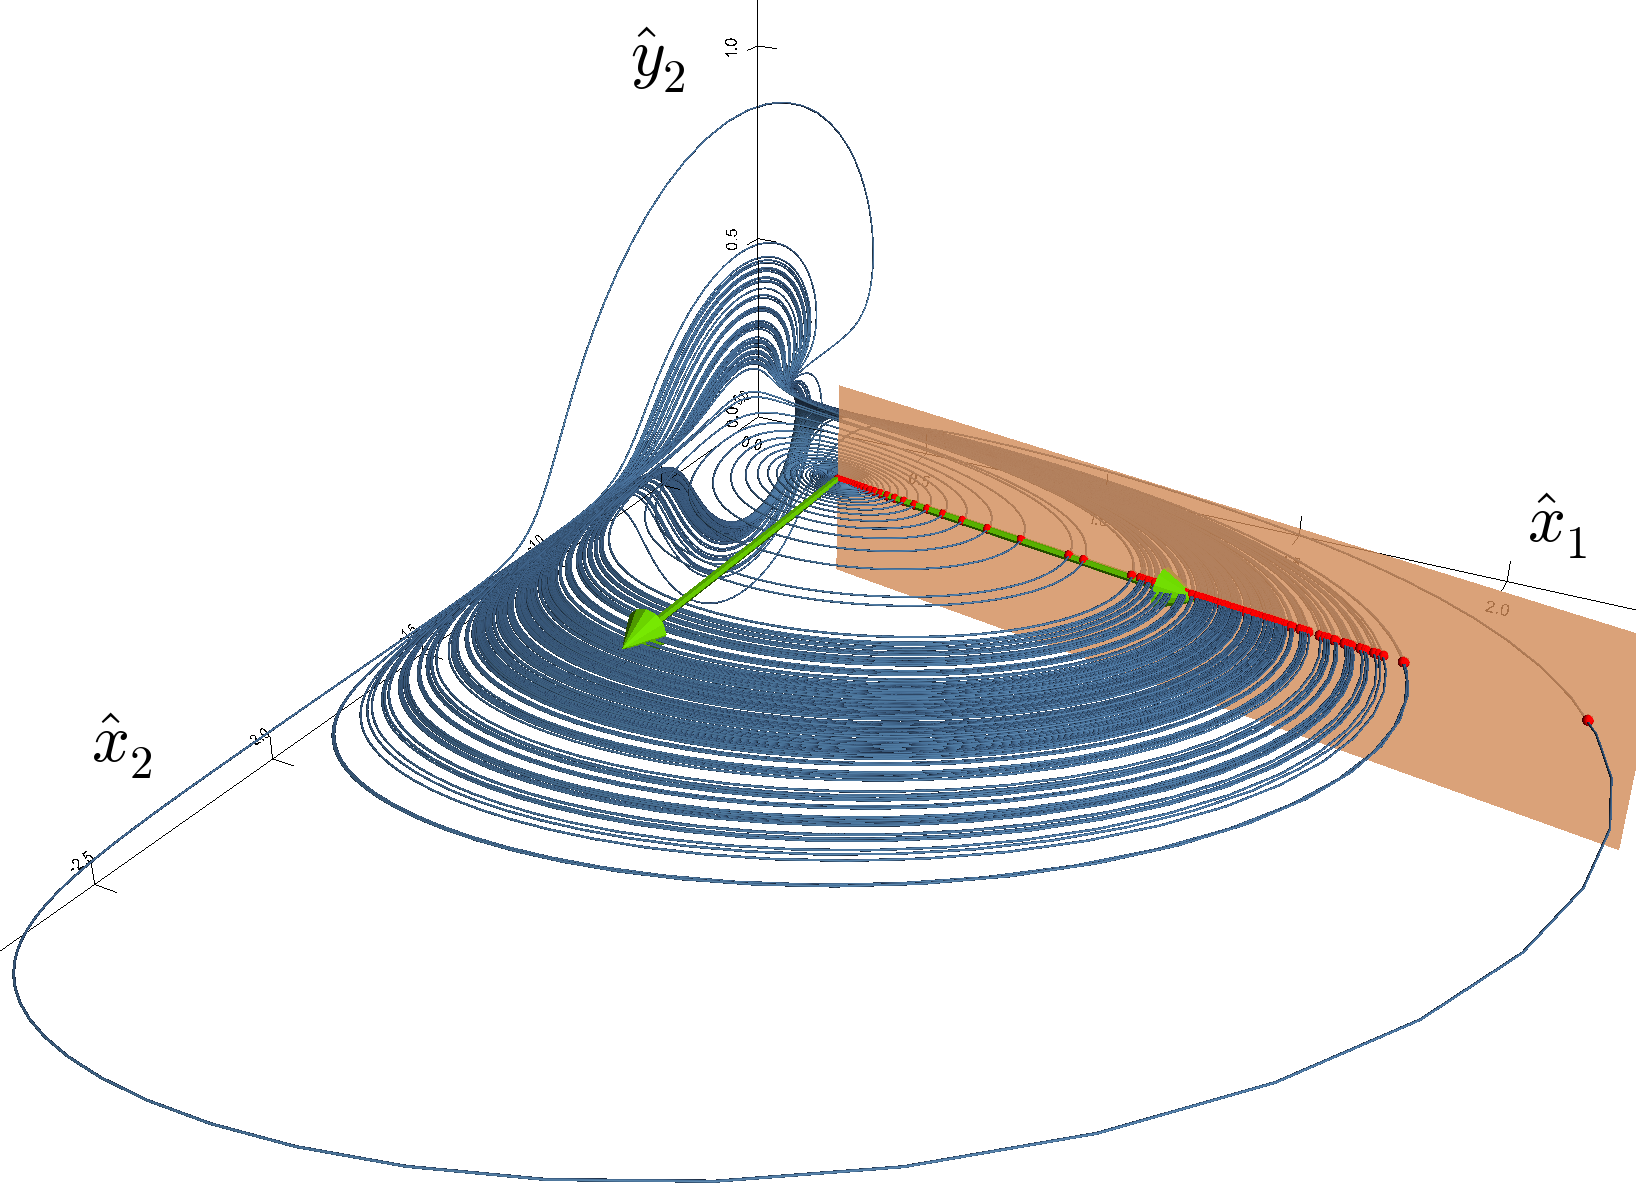
\includegraphics[width=0.45\textwidth]{BBpsecthd} \\
  (b) 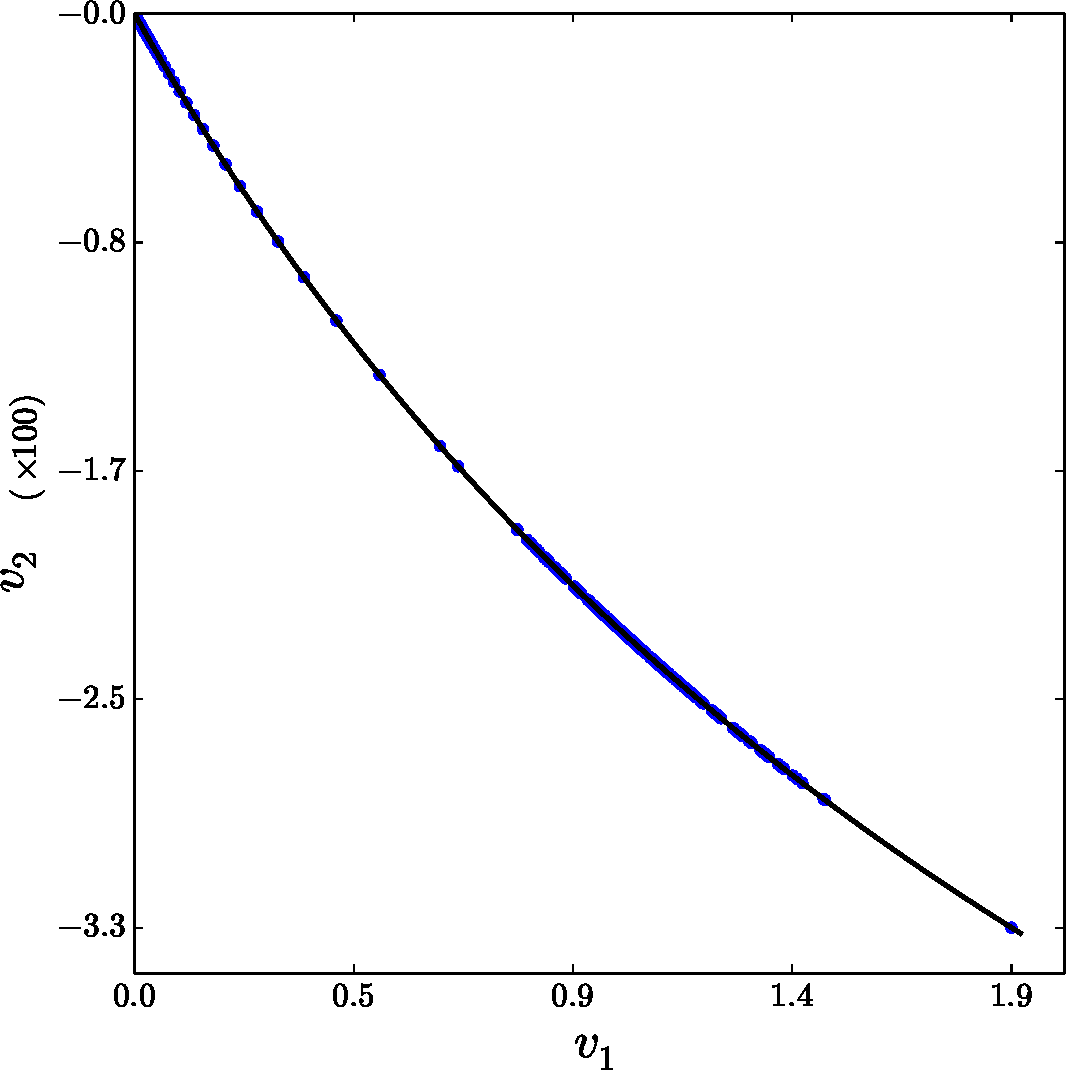
\includegraphics[width=0.20\textwidth]{BBpsectonslice}
  (c) 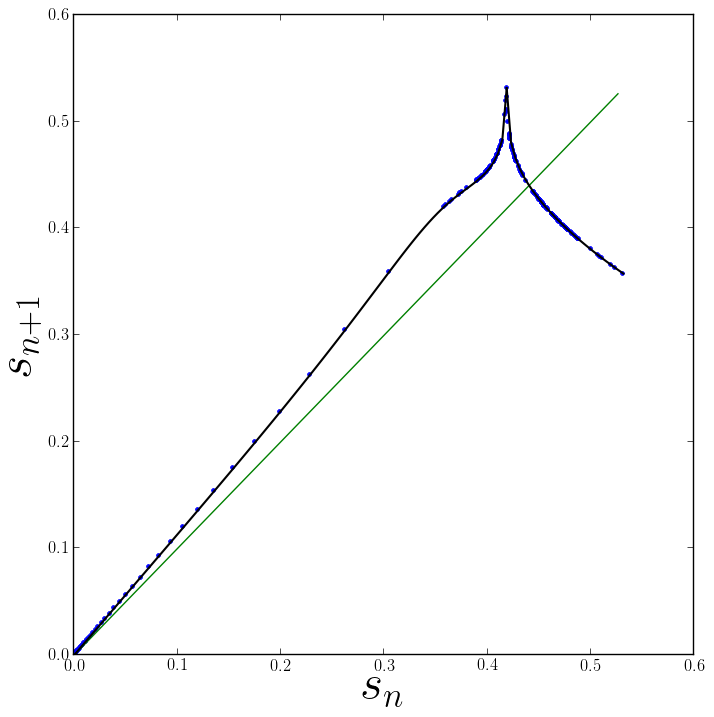
\includegraphics[width=0.20\textwidth]{BBretmaponslice} \\
  (d) 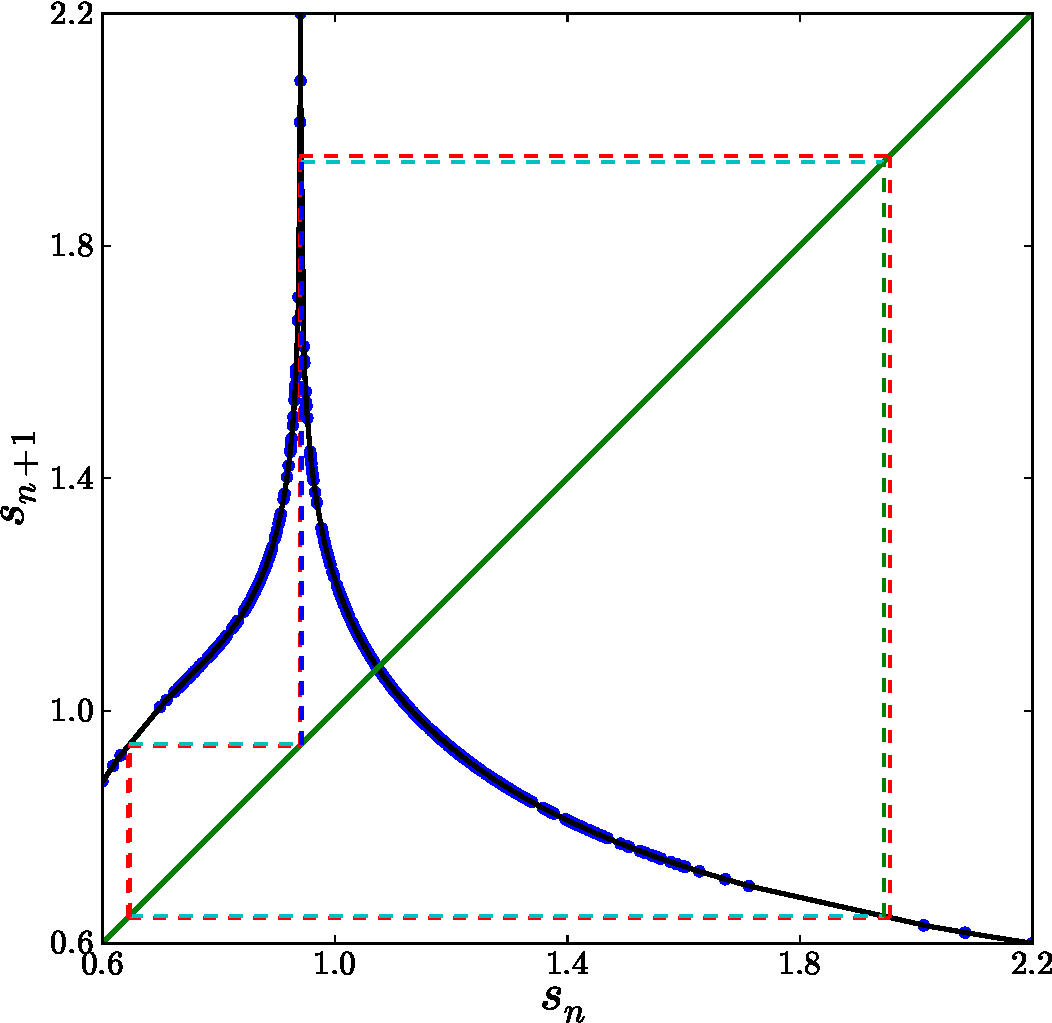
\includegraphics[width=0.45\textwidth]{BBretmaponsliceZoom}
\caption{(a) Symmetry reduced flow within the slice hyperplane (blue).
			Green arrows show the real and imaginary part of the unstable stability
			eigenvector $v_u$ of \REQV{}{}. A Poincar\'e section which includes
			$Im[v_u]$ is visualized as a transparent plane, and sections
			of the flow by the Poincar\'e section are marked with red.
		 (b) The Poincar\'e section which includes the \REQV{}{} and $v_u$ projected
			on to the basis within the plane shown in (a). Included is a
            transient trajectory initiated close to \REQV{}{}. Note that
		  	the vertical axis is magnified by $100$.
		 (c) The Poincar\'e arclength return map for the
		    Poincar\'e section (b).
		 (d) The return map without the transient points, framed by
            orbit of the critical point.
		 	Dashed lines show the 3-cycles \cycle{001} (red) and \cycle{011} (cyan).}
\label{fig:psectandretmap}
\end{figure}

Unimodal return map of \reffig{fig:psectandretmap} (d) lets us name the periodic orbits of the \twomode\ system according to their binary symbolic dynamics. Critical point of this map is at $s_C=0.98102264$, corresponding to the tip of the return map. Topological coordinate of the critical point, the kneading value, lets us determine the all admissible cycles of the system. For a detailed introduction to the symbolic dyanmics techniques we refer to \refref{DasBuch}. After determining the admissible cycles, we find candidates corresponding to the admissible symbol sequences from the return map, and feed them into a multiple shooting Newton solver (see Appendix \ref{s:newton}) to precisely determine the \rpo s. This way, we found the admissible cycles of the \twomode\ system upto the topological length 12. In \reffig{f-2modesrpofirst4} we show shortest $4$ of the \rpo s of the \twomode\ system within the first Fourier mode \slicePlane . As seen from \reffig{f-2modesrpofirst4}, trajectories of \cycle{001} and \cycle{011} almost overlap in a large region of the \statesp . This behavior is also manifested in the return map of \reffig{fig:psectandretmap} (d), where we have shown cycles \cycle{001} and \cycle{011} with red and cyan respectively. This is a general property of the \twomode\ cycles with odd topological lengths: They come in pairs with almost equal Floquet exponents, see \reffig{f-2modes-lambdaDist}.

\begin{figure}%[H]
\centering
 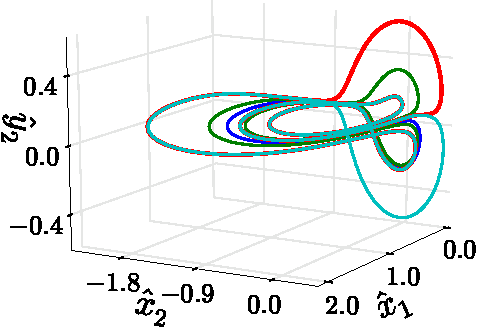
\includegraphics[width=0.45\textwidth]{2modesrpofirst4}
\caption{Shortest four \rpo s of the \twomode\ system: \cycle{1} (dark blue), \cycle{01} (green), \cycle{001} (red), \cycle{011} (cyan). Note that \rpo s \cycle{001} and \cycle{011} almost overlap everywhere except $\hat{x}_1 \approx 0$ .}
\label{f-2modesrpofirst4}
\end{figure}

\subsection{Dynamical Averages}
Spectrum of an observable, such as phase drift, or energy dissipation, of a dynamical system is dual to the spectrum of its periodic orbits by means of the classical trace formula \rf{DasBuch}:
\beq
\sum_{\alpha=0}^{\infty} \frac{1}{s-s_{\alpha}} = \sum_p T_p \sum_{r=1}^{\infty} \frac{e^{r(\beta A_p - s T_p)}}{\oneMinJ{r}} .
\ee{e-ClassicalTraceFormula}

\begin{figure}%[H]
\centering
 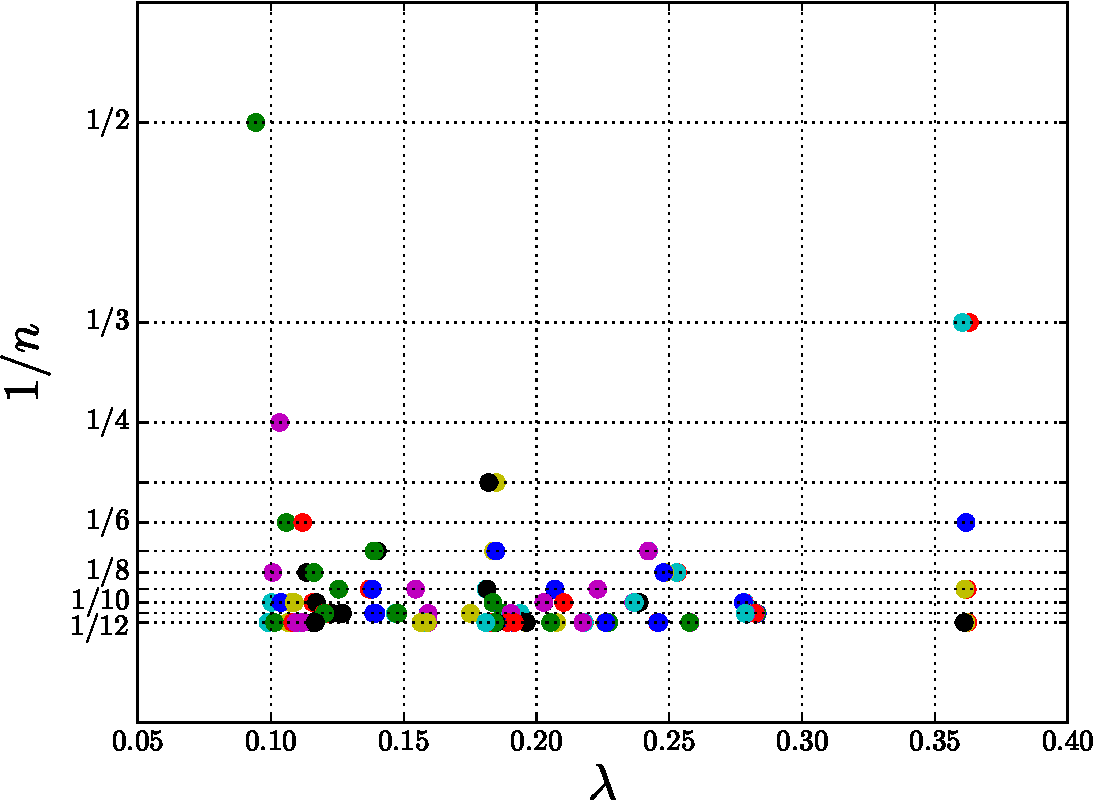
\includegraphics[width=0.45\textwidth]{2modes-lambdaDist}
\caption{Distribution of the leading Floquet exponents of \twomode\ cycles.}
\label{f-2modes-lambdaDist}
\end{figure}


Here, $s_{\alpha}$ are the eigenvalues of $\mathcal{A}$, the semigroup generator of the dynamical evolution of the observable $A$, outer sum on the RHS runs over the ``prime cycles'' of the system, $T_p$ is the period of the prime cycle $p$, $A_p$ is the value of the observable along the prime cycle, $\monodromy_p$ is the transverse (no marginal directions) monodromy matrix and $s$ and $\beta$ are auxilliary variables dual to the observable $A$ and time respectively. 

While the classical trace formula \refeq{e-ClassicalTraceFormula} manifests the essential duality between the spectrum of an observable and that of the periodic orbits, in practice, it is hard to work with since the eigenvalues are located at the poles of
\refeq{e-ClassicalTraceFormula}. For this reason, one expresses this duality equivalently as the following spectral determinant
\beq
    \det (s-\mathcal{A}) = \exp \left( - \sum_p \sum_{r=1}^{\infty}
                             \frac{1}{r} \frac{e^{r(\beta A_p - s T_p)}}{\oneMinJ{r}} \right)\, ,
\ee{e-SpectralDeterminant}
logarithmic derivative of which gives \refeq{e-ClassicalTraceFormula}. The spectral determinant \refeq{e-SpectralDeterminant} is easier to work with since the spectrum of $\mathcal{A}$, is now located at the zeros of \refeq{e-SpectralDeterminant}. Convergence of \refeq{e-SpectralDeterminant} is still not obvious. More insight is gained by approximating $\oneMinJ{r}$ by the product of expanding Floquet multipliers and then computing the $r$ sum in \refeq{e-SpectralDeterminant}. 
\bea
\oneMinJ{} &=& | (1 - \Lambda_{e,1})(1 - \Lambda_{e,2})... \continue 
			&&(1 - \Lambda_{c,1}) (1 - \Lambda_{c,2}) ... | \nonumber \\
			&\approx& \prod_e |\Lambda_e| = |\Lambda_p|,
\eea
where $|\Lambda_{e,i}| > 1$ and $|\Lambda_{c,i}| < 1$ are expanding and contracting Floquet multipliers respectively. After this approximation, $r$-sum in \refeq{e-SpectralDeterminant} becomes the Taylor expansion of natural logarithm and it can be compactly written as follows:
\beq
1 / \zeta = \prod_r (1 - t_p) \, \mbox{where}, \, t_p = \frac{1}{|\Lambda_p|} e^{\beta A_p - s T_p} z^{n_p} .
\ee{e-DynamicalZeta}
Where we inserted the `order tracking' term $z$. For complete binary symbolic dynamics, the dynamical zeta function \refeq{e-DynamicalZeta} can be brought into the `curvature expansion' form:
\bea
1 / \zeta &=& 1 - t_0 - t_1 - (t_{01} - t_0 t_1 )  \label{e-CycleExpansion} \\
		  && - [(t_{011} - t_{01}t_1) + (t_{001} - t_{01} t_0)] - ... \continue
		  &=& 1 - \sum_f t_f - \sum_n \hat{c}_n \label{e-CurvatureExpansion}.
\eea
In the curvature expansion \refeq{e-CurvatureExpansion}, we grouped the contributions to the dynamical zeta function as `fundamental' contributions $t_f$ and `curvature' corrections. One expects the curvature corrections to be small since the longer prime cycles are `shadowed' by the combination of the shorter ones, the `pseudocycles'. 

For complete binary symbolic dynamics, the only fundamental contributions to the dynamical zeta function are the cycles with topological length $1$, see \refeq{e-CurvatureExpansion}. This is not the case for any map since in general there might be non-trivial pruning rules, hence longer cycles can appear unshadowed. The Poincar\'e return map of \reffig{fig:psectandretmap} (d) is such a map with non-trivial pruning rules, however, note that cycles \cycle{001} and \cycle{011} passes very close to the tip of the cusp, the critical point, in \reffig{fig:psectandretmap} (d). This observation motivates us to approximate the return map of \reffig{fig:psectandretmap} (d), as if its tip is located at $s = 0.97986453$, where the cycle \cycle{001} lands, and omit the contributions above this point. We will refer this approximation as the `finite grammar approximation' since by doing it, we obtain single pruning rule; that is the symbol sequence $00$ is not allowed. This grammar is known as the `golden mean' pruning and a complete binary symbolic dynamics can be converted to the golden mean symbolic dynamics by substitution $0 \rightarrow 01$. We can write the dynamical zeta function for the golden mean pruned symbolic dynamics by replacing $0$s in \refeq{e-CycleExpansion} by $01$:
\bea
1 / \zeta &=& 1 - t_{01} - t_1 - (t_{011} - t_{01} t_1 ) \label{e-GoldenMeanCycleExpansion}\\
		  && - [(t_{0111} - t_{011}t_1) + (t_{01011} - t_{01} t_{011} ) ] - ... \nonumber
\eea
Note that all the contributions longer than topological length $2$ to the golden mean dynamical zeta function are in form of shadowing combinations. However, as we shall see, they are not small.

While dynamical zeta functions are useful for investigating the convergence properties, they are not exact, and their computational cost is same with that of the exact spectral determinants. For this reason, we will expand the spectral determinant \refeq{e-SpectralDeterminant} ordered in the topological length of cycles and pseudocycles as follows:
\beq
    \det (s-\mathcal{A}) =   \prod_p \exp \left( - \sum_{r=1}^{n_p r < N}
                             \frac{1}{r} \frac{e^{r(\beta A_p - s T_p)} 
                                          }{\oneMinJ{r}} z^{n_p r} \right) \, .
\ee{e-SpectralDeterminantExp}
This is the form that we use to compute the spectral determinant. For each prime cycle, we compute the sum term in \refeq{e-SpectralDeterminantExp} truncated at the expansion order $N$, and then expand the exponential upto order $N$, and multiply this expansion with the contributions from previous cycles and drop terms with order greater than $N$. This way, we obtain the $N^{th}$ order spectral determinant \refeq{e-SpectralDeterminant}. Let us denote the resultant series after setting $z=1$ as
\beq
    F_N(s, \beta ) = 1 - \sum_{n=1}^{N} Q_n(s, \beta ) \, . 
    \label{e-NthOrderSpectDet}
\eeq
Leading $0$ of $F_N(s, 0)$, $s_0$, corresponds to the leading eigenvalue of the Perron-Forbenius operator, $\gamma_0 = - s_0$, which can be interpreted as the `escape rate'. We expect the escape rate to be small, ideally zero, if the cycle expansion is good.
After finding $s_0$, we can compute the dynamical averages as follows:
Mean period:
\bea
    \langle T \rangle_N &=& \left. \frac{\partial F_N}{\partial s} 
                            \right|_{\beta=0, s=s_0} \, , \label{e-AveragePeriod} \\
    \langle A \rangle_N &=& - \left. 
                              \frac{\partial F_N}{\partial \beta} 
                              \right|_{\beta=0, s=s_0} \, ,   \label{e-AvgA} \\
    \langle (A - \langle A \rangle )^2 \rangle_N 
    &=& - \left. \frac{\partial^2 F_N}{\partial \beta^2} \right|_{\beta=0, 
                                                  s=s_0} \, , \label{e-AvgSigma} \\
    \langle a \rangle_N &=& - \frac{1}{\langle T \rangle_N} \left. 
                              \frac{\partial F_N}{\partial \beta} 
                              \right|_{\beta=0, s=s_0} \, ,   \label{e-Avga} \\
    \langle (a - \langle a \rangle )^2 \rangle_N 
    &=& - \frac{1}{\langle T \rangle_N} \left. \frac{\partial^2 F_N}{\partial \beta^2} \right|_{\beta=0, 
                                                                    s=s_0} \, \label{e-Avgsigma} .                        
\eea
Here, $\langle T \rangle_N$ is average cycle period, $A$ denotes an observable that is ``additive'' along the trajectories, in other words, that satisfies semi-group property; and $a$ a is the rate of that observable. For example, for $A = \phi$, \refeq{e-AvgA} yields the ``average phase shift per cycle'', whereas \refeq{e-Avga} yields ``average phase speed''. Variances \refeq{e-AvgSigma} and \refeq{e-Avgsigma} are respectively interpreted similarly as the ``variance per cycle'' and ``variance rate'' of an observable.

We computed escape rate $\gamma$, average cycle period $\langle T \rangle$, leading Lyapunov exponent $\lambda$, average phase speed $\langle \dot{\phi} \rangle$ and the phase diffusion constant $D$ of the \twomode\ system using cycle averaging formulas \refeqs{e-AveragePeriod}{e-Avgsigma}. We listed our findings with respect to the increasing expansion order in \reftab{t-DynamicalAverages} and \reftab{t-DynamicalAveragesNoGrammar}. While in \reftab{t-DynamicalAverages} we used the finite grammar approximation, in \reftab{t-DynamicalAveragesNoGrammar} we input all the cycles we found to the calculation. 

\begin{table}
	\begin{tabular}{c|c|c|c|c|c}
	 $N$ & $\gamma$ & $\langle T \rangle$ & $\lambda$ & $\langle \dot{\phi} \rangle$ & $D$ \\ 
	\hline
	1 & 0.24983007 & 3.64151210 & 0.10834935 & 0.02223518 & 0.00090019 \\ 
 	2 & -0.01159743 & 5.89675999 & 0.10302904 & -0.14242535 & 0.22615040 \\ 
 	3 & 0.02744646 & 4.72713874 & 0.11849781 & -0.14916163 & 0.22541882 \\ 
 	4 & -0.00445545 & 6.23866097 & 0.10631075 & -0.22271184 & 0.54199883 \\ 
 	5 & 0.00068106 & 5.89674866 & 0.11842709 & -0.19506985 & 0.47091930 \\ 
 	6 & 0.00068491 & 5.89688492 & 0.11820055 & -0.21660997 & 0.64918118 \\ 
 	7 & 0.00063044 & 5.90316812 & 0.11835165 & -0.18083296 & 0.51935080 \\ 
 	8 & 0.00071488 & 5.89189180 & 0.11827587 & -0.21129228 & 0.78673581 \\ 
 	9 & 0.00072867 & 5.88975993 & 0.11826879 & -0.19203222 & 0.70977900 \\ 
 	10 & 0.00072808 & 5.88986409 & 0.11826793 & -0.20302879 & 0.90493496 \\ 
 	11 & 0.00072790 & 5.88989901 & 0.11826783 & -0.19453187 & 0.86683629 \\ 
 	\end{tabular}
	\caption{Cyle expansion estimates of the escape rate $\gamma$, average cycle period $\langle T \rangle$, Lyapunov exponent $\lambda$, average phase velocity $\langle \dot{\phi} \rangle$ and the diffusion coefficient $D$ with respect to the expansion order $N$ .}
	\label{t-DynamicalAverages}
\end{table}
\begin{table}
	\begin{tabular}{c|c|c|c|c|c}
	 $N$ & $\gamma$ & $\langle T \rangle$ & $\lambda$ & $\langle \dot{\phi} \rangle$ & $D$ \\ 
	\hline
	1 & 0.24982996 & 3.64151221 & 0.10834917 & 0.02223518 & 0.00090019 \\ 
 	2 & -0.01159761 & 5.89676053 & 0.10302891 & -0.14242516 & 0.22615014 \\ 
 	3 & 0.02261469 & 4.88995874 & 0.13055574 & -0.16698925 & 0.28645997 \\ 
 	4 & -0.00606560 & 6.24822611 & 0.11086469 & -0.22623282 & 0.55402655 \\ 
 	5 & 0.00091264 & 5.77716415 & 0.11812034 & -0.19839015 & 0.47840111 \\ 
 	6 & 0.00026210 & 5.83645342 & 0.11948918 & -0.21788301 & 0.65393430 \\ 
 	7 & 0.00001771 & 5.86382098 & 0.12058951 & -0.18565119 & 0.55022944 \\ 
 	8 & 0.00011328 & 5.85110445 & 0.12028459 & -0.21480977 & 0.80768111 \\ 
 	9 & 0.00017071 & 5.84222727 & 0.12010579 & -0.19376222 & 0.72685211 \\ 
 	10 & 0.00015683 & 5.84466944 & 0.12014022 & -0.20501316 & 0.92174228 \\ 
 	\end{tabular}
	\caption{Cyle expansion estimates of the escape rate $\gamma$, average cycle period $\langle T \rangle$, Lyapunov exponent $\lambda$, average phase velocity $\langle \dot{\phi} \rangle$ and the diffusion coefficient $D$ with respect to the expansion order $N$ .}
	\label{t-DynamicalAveragesNoGrammar}
\end{table}


We motivated our finite grammar approximation by expecting a fast convergence after second order in the cycle expansion, however,
this is not the case. The reason is, as we mentioned before, that the curvature corrections of \refeq{e-GoldenMeanCycleExpansion} are not small. This is due to the fact that the Floquet exponent of the cycle \cycle{011} (marked cyan at $1/3$ line of \reffig{f-2modes-lambdaDist}), is much larger than the rest of the set that appears in the cycle expansion, and since the cycle contributions are weighted by the inverse Floquet multipliers, $t_{011}$ almost cancels every shadowing combination it appears. Hence the curvature corrections in which $t_{011}$ appears as a shadowing orbit, are not small. However, we still get a better convergence comparing to the case where we include all cycles in the calculation. \refTab{t-DynamicalAverages} and \reftab{t-DynamicalAveragesNoGrammar} show that when the expansion order is $10$, the Lyapunov exponents converges with a $6$ digits in the finite grammmar calculations, whereas it has $4$ digit convergence in the case where we included all cycle contributions.

In order to compare with the cycle averages, we numerically estimated the leading Lyapunov exponent of the \twomode\ system using the method of Wolf \etal\ \ref{WolfSwift85}. This procedure was repeated 100 times for different initial conditions, yielding a mean estimate of $\lambda_{Numerical} = 0.1198 \pm 0.0008$. While the finite grammar estimate $\lambda_{FG} = 0.118268$ is within $1\%$ range of this value, the full cycle expansion agrees with the numerical estimate. This is not surprising, since in the finite grammar approximation, we discard the most unstable cycles, thus, we obtain a slightly smaller Lyapunov exponent while obtaining a better convergence. 